\section{Ray-Marching}
Eine weitere Möglichkeit, biologisch inspirierte Strukturen zu erzeugen, sind Fraktale.
Fraktale sind selbstähnliche Strukturen, die immer feiner aufgelöst werden können.
Es ist möglich, diese Fraktale als Meshes zu modellieren und auf herkömmliche Weise zu rendern.
Allerdings ist dies nur bis zu einem gewissen Punkt praktikabel.
Ein alternatives Verfahren zum Rendern der Strukturen ist das Ray-Marching, bei welchem die Strukturen nicht als Meshes, sondern als implizite Funktionen dargestellt werden \cite{wikipedia_raymarching}.

\begin{figure}[!htbp]\centering
    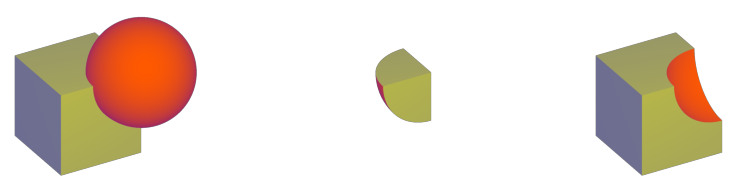
\includegraphics[width=0.4\textwidth]{csg_operations.png}
    \caption{\cite{fotonixx_csg}}
    \label{fig:bool_ops}
\end{figure}

\subsection{Darstellung von Objekten} \label{sec:ray_marching:objects}
Die Darstellung von Objekten erfolgt mittels \emph{Signed Distance Functions} (SDF).
Diese Funktionen geben für einen bestimmten Punkt im Raum den Abstand zur Oberfläche eines Objekts an.
Die Funktionen können sowohl positive als auch negative Werte zurückgeben, je nachdem, ob sich der Punkt innerhalb oder außerhalb der Struktur befindet.
Ein Beispiel für eine primitive Funktion ist die einer Kugel im Ursprung mit einem Radius von 1.
Diese kann als $||p||_2 - r$ beschrieben werden, wobei $||p||_2$ der euklidische Abstand des Punktes $p$ zum Ursprung und $r$ der Radius der Kugel ist.
Wenn $p$ innerhalb der Kugel liegt, ist der Abstand negativ, wenn $p$ außerhalb der Kugel liegt, ist der Abstand positiv und wenn $p$ genau auf der Oberfläche der Kugel liegt, ist der Abstand 0.
Für eine Vielzahl von primitiven und komplexeren Strukturen können solche SDFs gefunden werden \cite{iquilezles_distfunctions}.
Befinden sich nun zwei oder mehr Objekte im Raum, so können diese durch verschiedene Operationen miteinander verknüpft werden.
Wenn das Minimum der beiden Funktionen gebildet wird, ergibt sich eine neue Funktion, die den Abstand zum nächstgelegenen der beiden Objekte angibt.
Beim Maximum der beiden Funktionen, ergibt sich eine Funktion, die den Schnitt der beiden Objekte beschreibt.
Es ist auch möglich, ein Objekt von dem anderen zu subtrahieren, indem das Maximum eines Objekts zusammen mit dem negativen Wert des anderen Objekts, das von dem ersten Objekt abgezogen werden soll, gebildet wird.
\autoref{fig:bool_ops} zeigt die Vereinigung und den Schnitt eines Würfels mit einer Kugel sowie das Ergebnis, wenn die Kugel von dem Würfel subtrahiert wird.


\subsection{Ray-Marching-Algorithmus}
Zum Darstellen der Objekte wird ein Ray-Marching-Algorithmus verwendet.
Dabei wird für jedes Pixel des Bildes ein Strahl von der Kamera in die Szene geschickt.
Mit Hilfe der SDF kann der Abstand zum nächsten Objekt bestimmt werden.
Obwohl nicht bekannt ist, wo sich das nächstgelegene Objekt befindet, kann sichergestellt werden, dass der Strahl nicht zu weit in die Szene hineingeschickt wird.
Der Strahl läuft dann um den berechneten Abstand weiter in die vorgegebene Richtung und von diesem Punkt aus wird erneut der Abstand zum nächsten Objekt berechnet.
Dieser Vorgang wird iterativ wiederholt, bis entweder ein oberes Limit an Iterationen erreicht ist, eine maximal zulässige Distanz überschritten wurde oder der Abstand zum nächsten Objekt kleiner als ein vorgegebenes Minimum ist.
Wenn dieses Minimum erreicht ist, wird angenommen, dass der Strahl auf ein Objekt trifft.
Wenn das obere Limit der Iterationen erhöht oder das Minimum verringert wird, erhöht sich die Genauigkeit des Algorithmus, wodurch die Objekte höher aufgelöst werden, aber auch die Laufzeit steigt.

\begin{figure}[!htbp]\centering
    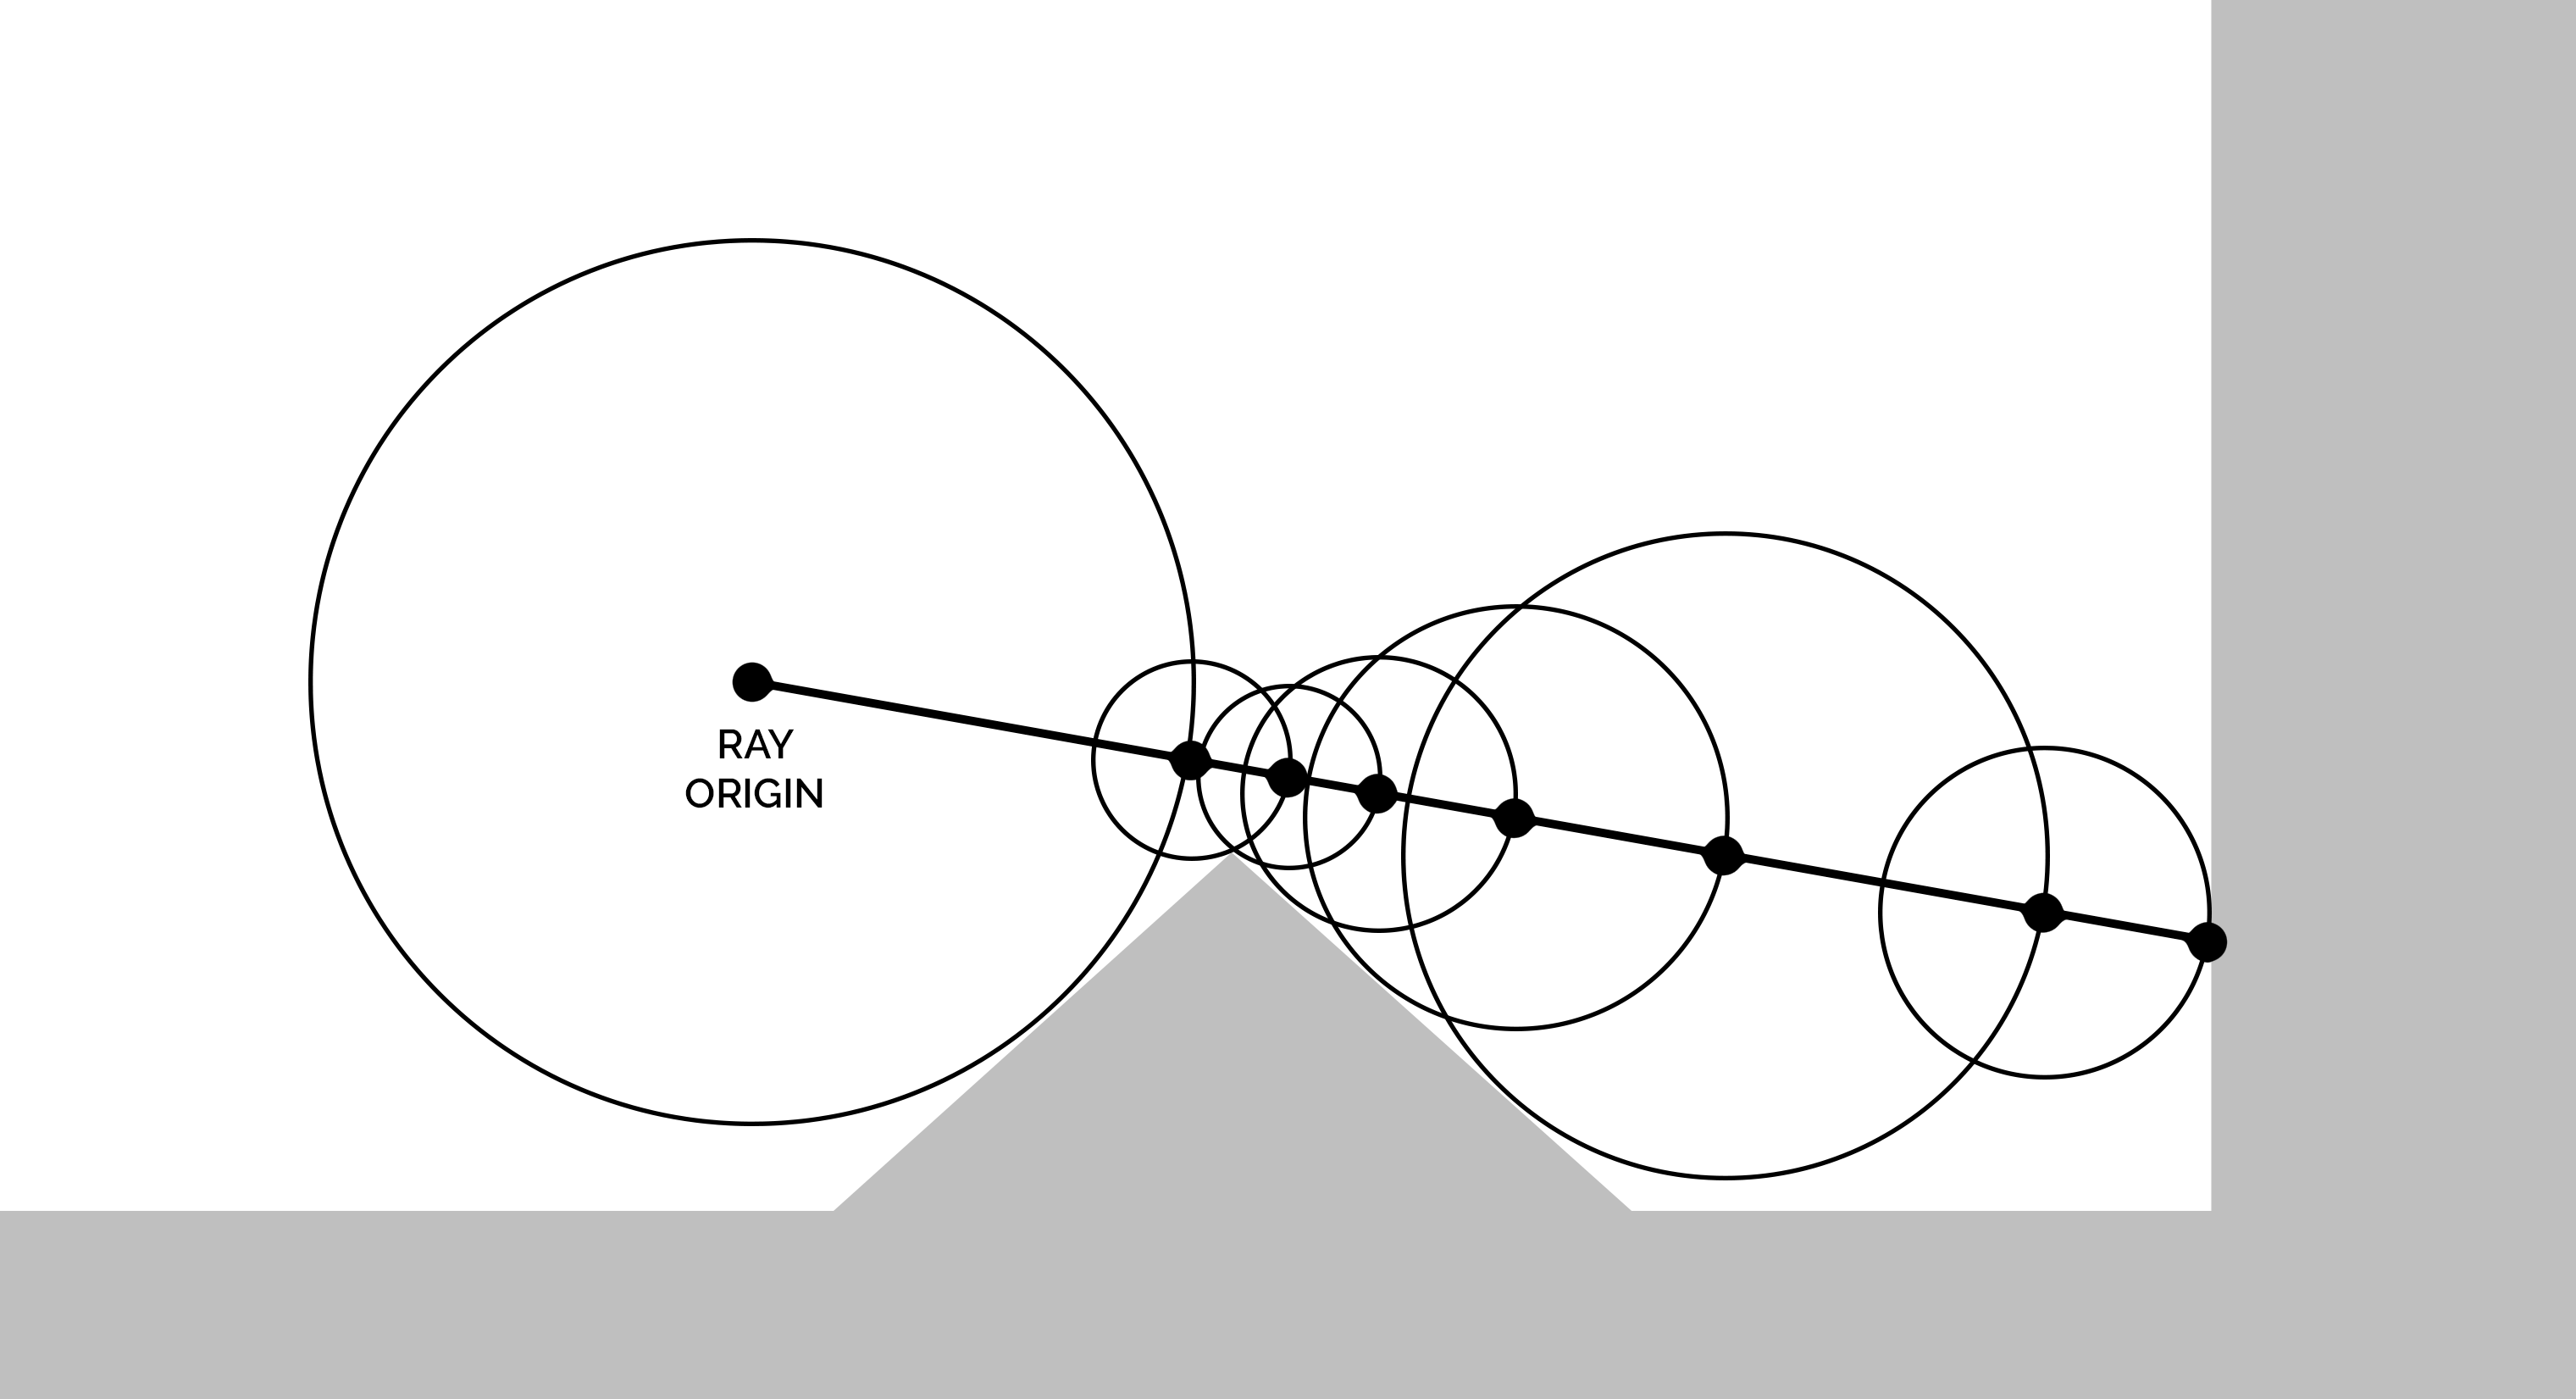
\includegraphics[width=0.5\textwidth - 7.82454pt]{Visualization_of_SDF_ray_marching_algorithm.png}
    \caption{Visualisierung des Ray-Marching-Algorithmus. \cite{wikimedia_sdf}}
    \label{fig:ray_marching}
\end{figure}

\begin{figure}[!htbp]\centering
    \begin{subfigure}[t]{0.2\textwidth}
        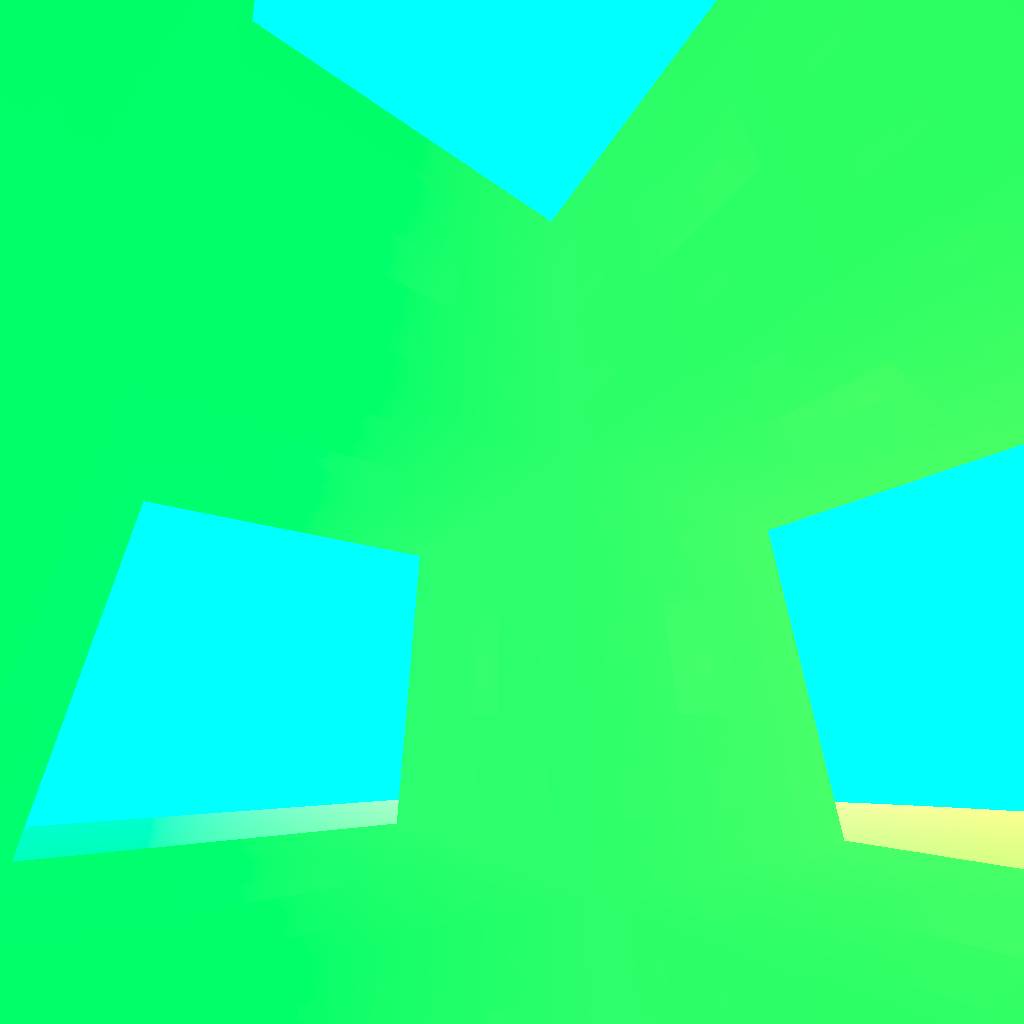
\includegraphics[width=\textwidth]{Viewer0.png}
        \caption{Keine Beleuchtung}
        \label{fig:lighting:none}
    \end{subfigure}
    \hfill
    \begin{subfigure}[t]{0.2\textwidth}
        \centering
        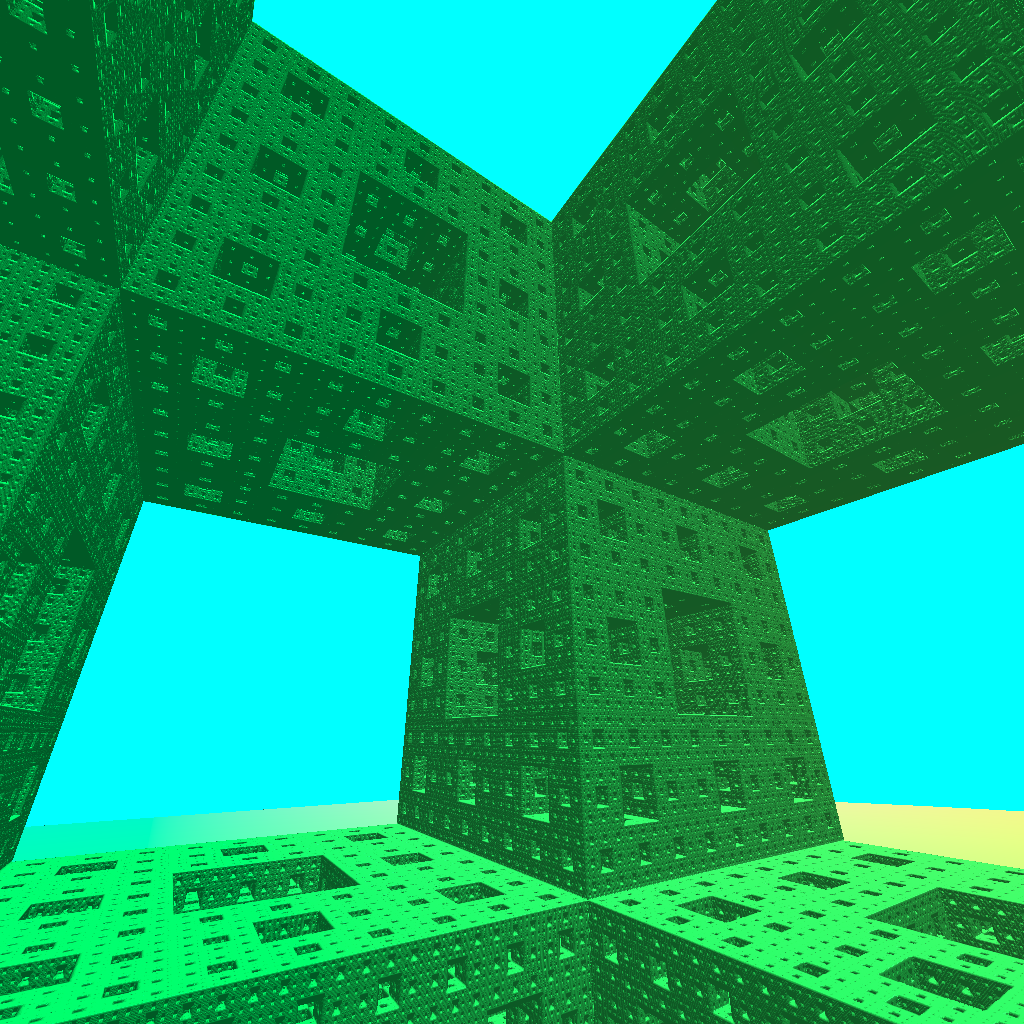
\includegraphics[width=\textwidth]{Viewer1.png}
        \caption{Phong-Beleuchtung}
        \label{fig:lighting:phong}
    \end{subfigure}
    \hfill
    \begin{subfigure}[t]{0.2\textwidth}
        \centering
        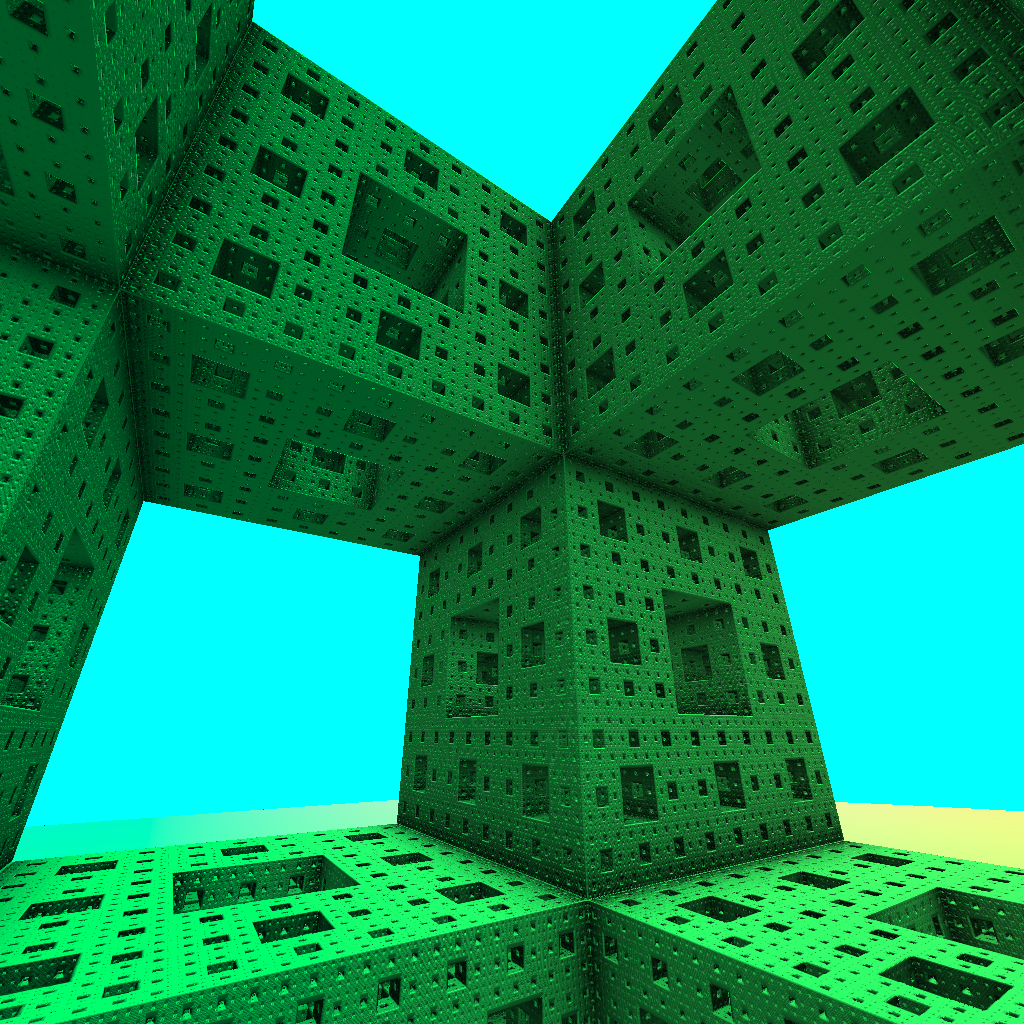
\includegraphics[width=\textwidth]{Viewer2.png}
        \caption{Ambient Occlusion}
        \label{fig:lighting:ao}
    \end{subfigure}
    \hfill
    \begin{subfigure}[t]{0.2\textwidth}
        \centering
        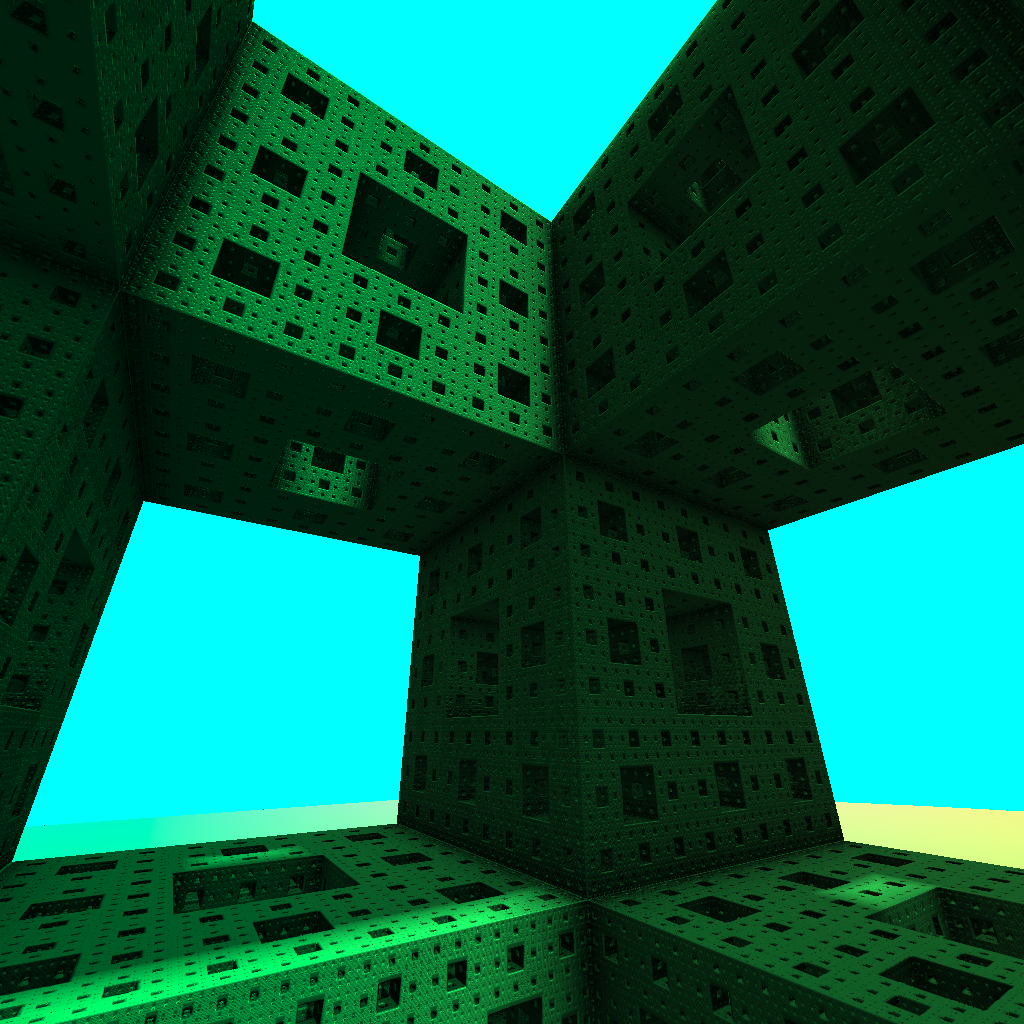
\includegraphics[width=\textwidth]{Viewer3.png}
        \caption{Soft Shadows}
        \label{fig:lighting:soft}
    \end{subfigure}
    \caption{Inkrementelles Hinzufügen von Beleuchtungseffekten}
    \label{fig:lighting}
\end{figure}

\subsection{Licht und Schatten}
Trifft nun ein Strahl auf ein Objekt, so kann für diesen Punkt ein Beleuchtungsmodell ausgewertet werden.
Wird dafür beispielsweise das Phong-Beleuchtungsmodell verwendet, so wird dafür die Normale an dem Punkt benötigt.
Für einfache Objekte wie Kugeln oder Flächen kann diese Normale unkompliziert bestimmt werden, für komplexere Strukturen kann dies jedoch schwierig sein.
Die Normale eines Punktes kann mit dem Gradienten der SDF an diesem Punkt bestimmt werden.
Dies kann numerisch approximiert werden, indem die SDF um den Punkt herum in alle drei Richtungen mit einem kleinen Abstand ermittelt und der Abstand zum Punkt berechnet wird.
Dies entspricht der Bestimmung des Gradienten der SDF an diesem Punkt, womit die Normale an diesem Punkt bestimmt werden kann.
Ist die Normale an dem Punkt bekannt, so kann das bekannte Phong-Beleuchtungsmodell verwendet werden, um die Beleuchtung an dem Punkt auszuwerten, wie in \autoref{fig:lighting:phong} zu sehen ist.

Mithilfe der Normalen lässt sich ebenfalls Ambient Occlusion bestimmen.
Dazu wird von einem Oberflächenpunkt aus entlang der Richtung der Normale ein Strahl in die Szene geschickt und dabei der Abstand zum nächsten Objekt bestimmt.
Dies geschieht für eine feste Anzahl von Schritten, wobei in jedem Schritt die Weite des Strahls vergrößert wird.
Dabei werden die ermittelten Entfernungen und die vom Strahl zurückgelegte Distanz aufsummiert.
Wenn kein anderes Objekt in der Nähe liegt, ist die Summe der Objektentfernungen $S$ gleich der Summe der zurückgelegten Distanzen $M$, da die SDF in jedem Schritt den Abstand zum Ausgangspunkt zurückgeben würde.
Wenn ein anderes Objekt in der Nähe ist, wäre $S$ kleiner als $M$.
$S \div M$ ergibt dann einen Wert zwischen 0 und 1, der als Ambient Occlusion-Wert verwendet werden kann, indem er mit dem Farbwert des Punktes multipliziert wird.
Dieses Verfahren kann verfeinert werden, indem weiter entfernte Distanzen weniger stark gewichtet werden \cite{zucconi_ao}.
Das Ergebnis ist in \autoref{fig:lighting:ao} dargestellt.

Eine einfache Möglichkeit Schatten zu erzeugen besteht darin, von jedem Punkt auf der Oberfläche einen Strahl zur Lichtquelle zu senden und zu überprüfen, ob dieser Strahl auf ein Objekt trifft.
Wenn der Strahl auf ein Objekt trifft, liegt der Punkt im Schatten und es wird ein dunklerer Farbwert verwendet.
Dieses Verfahren erzeugt scharfe Schatten, die jedoch nicht immer erwünscht sind.
Wenn ein Strahl auf dem Weg zwischen dem Punkt und der Lichtquelle ein Objekt nur knapp verfehlt, könnte dieser im Halbschatten liegen, um ein weicheres Schattenbild zu erzeugen.
Für jeden Schritt der Ray-Marching-Iteration zwischen Punkt und Lichtquelle kann ein Halbschatten-Faktor bestimmt werden.
Dieser ergibt sich aus dem Wert der SDF des aktuellen Punktes der Iteration, der ins Verhältnis zur Distanz zum Ausgangspunkt gesetzt wird, sodass weiter entfernte Objekte weniger stark gewichtet werden.
Von den bestimmten Halbschatten-Faktoren entlang des Strahls wird dann der kleinste Wert verwendet, um den Farbwert des Punktes zu bestimmen.
Aufgrund der geringeren Gewichtung der Werte für weiter entfernte Objekte entsteht außerdem der Effekt, dass die Schatten weicher werden, je weiter sie von dem Objekt entfernt sind und umgekehrt \cite{iquilezles_rmshadows}.
Dieser Effekt ist in \autoref{fig:shadows:soft} dargestellt.

\begin{figure}[!htbp]\centering
    \begin{subfigure}[t]{0.2\textwidth}
        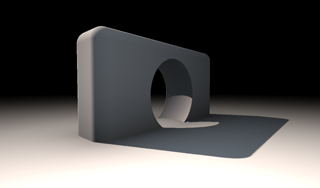
\includegraphics[width=\textwidth]{gfx12.png}
        \caption{Hard Shadow}
        \label{fig:shadows:hard}
    \end{subfigure}
    \hfill
    \begin{subfigure}[t]{0.2\textwidth}
        \centering
        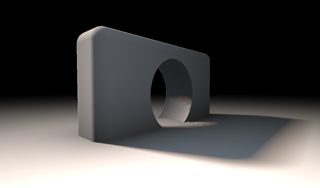
\includegraphics[width=\textwidth]{gfx08.png}
        \caption{Soft Shadow}
        \label{fig:shadows:soft}
    \end{subfigure}
    \caption{\cite{iquilezles_rmshadows}}
    \label{fig:shadows}
\end{figure}


\subsection{Fraktalstrukturen}
Um fraktalartige Strukturen zu erstellen, können SDFs verwendet werden, die sich unendlich oft wiederholen.
Eine Kugel, die mit einer SDF dargestellt wird und deren untere linke Ecke im Ursprung liegt und einen Radius von 1 hat, ist in \autoref{fig:sphere:simple} dargestellt.
Die SDF nimmt einen Punkt im Raum als Eingabe und gibt den Abstand zu der Oberfläche der Kugel zurück.
Dieser Punkt im Raum ist der aktuelle Punkt der Ray-Marching-Iteration.
Wenn auf die x-, y- und z-Koordinate dieses Punktes der Modulo-Operator mit beispielsweise 5 angewendet wird, liegen die jeweiligen Werte immer zwischen 0 und 5.
Das bedeutet, dass wenn der Strahl auf der x-Achse nach rechts die 5 überschreiten würde, er dies nicht tut und stattdessen von links wieder bei 0 anfängt.
Geschieht dies für alle Achsen, ergibt sich ein impliziter Kasten mit einer Kantenlänge von 5.
Alle Objekte innerhalb dieses Kastens werden aufgrund der Modulo-Operation unendlich oft in alle Richtungen wiederholt.
\autoref{fig:sphere:inf} zeigt, wie dies für eine Kugel aussehen kann.
Wenn dies nur in einer Achsenrichtung geschehen soll, kann der Modulo-Operator nur auf eine Achse angewendet werden.

\begin{figure}[!htbp]\centering
    \begin{subfigure}[t]{0.2\textwidth}
        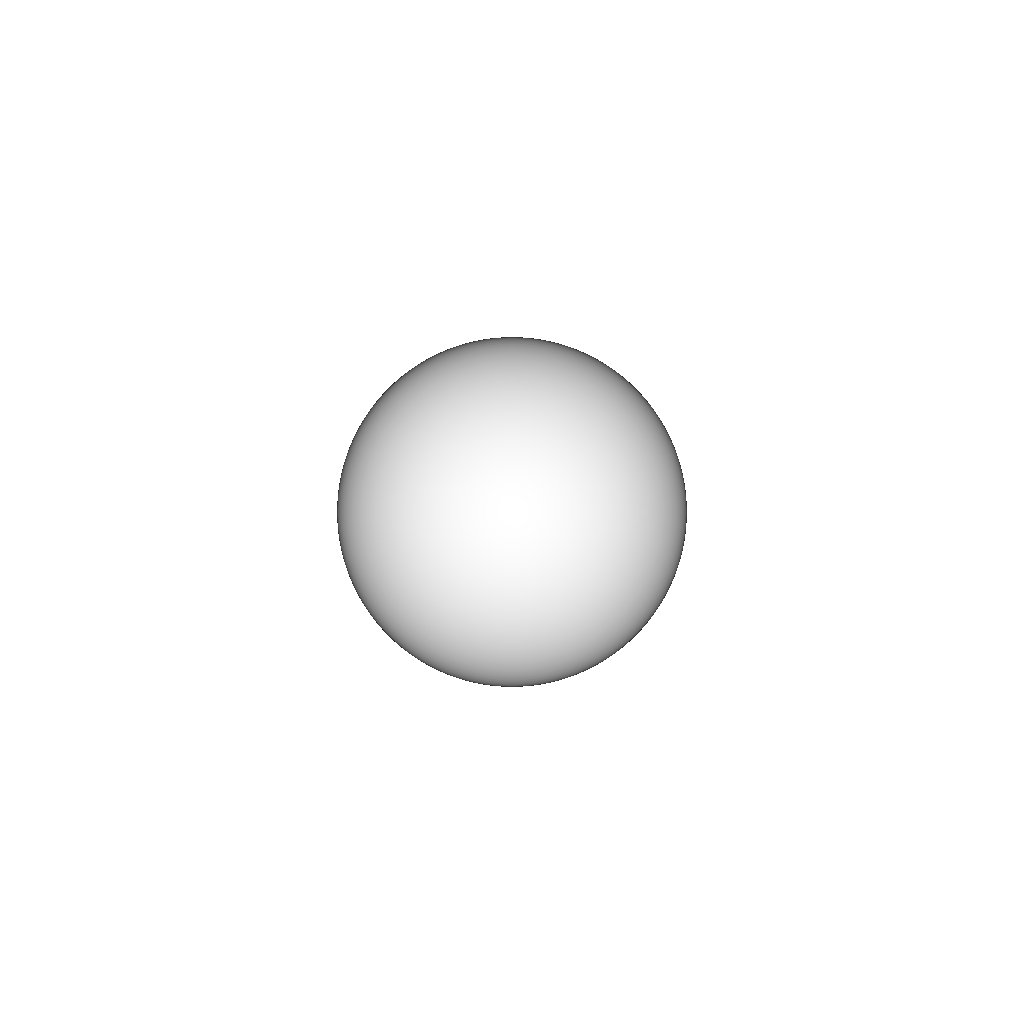
\includegraphics[width=\textwidth]{sphere0.png}
        \caption{}
        \label{fig:sphere:simple}
    \end{subfigure}
    \hfill
    \begin{subfigure}[t]{0.2\textwidth}
        \centering
        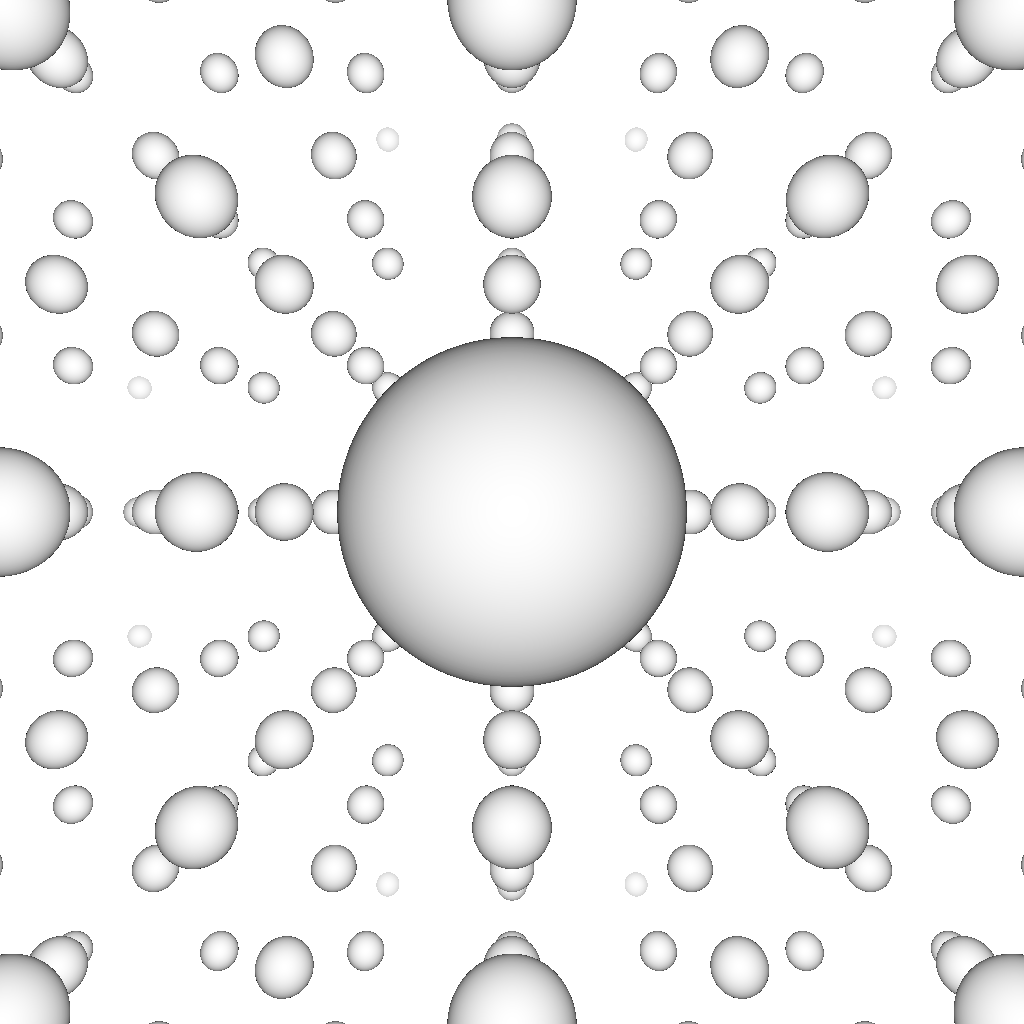
\includegraphics[width=\textwidth]{sphere1.png}
        \caption{}
        \label{fig:sphere:inf}
    \end{subfigure}
    \caption{}
    \label{fig:sphere}
\end{figure}


Der \textit{Menger-Sponge} ist ein Beispiel für eine fraktale Struktur, die sich mit den vorgestellten Methoden dargestellt lässt.
Dazu wird zunächst mit einem Würfel begonnen.
Von diesem wird dann ein Kreuz, wie in \autoref{fig:menger:cross0} zu sehen, mithilfe der in Kapitel \ref{sec:ray_marching:objects} beschriebenen Operationen abgezogen.
Anschließend wird das Kreuz auf $1/3$ seiner vorherigen Größe skaliert und mit dem zuvor erklärten Verfahren in alle Richtungen unendlich oft wiederholt und ebenfalls von dem Würfel abgezogen.
Dieses Verfahren wird nun iterativ wiederholt, bis der Menger-Sponge die gewünschte Auflösung erreicht hat.
\autoref{fig:menger} zeigt dieses iterative Verfahren.
Dabei ist in grün die aktuelle Iteration zu sehen und in rot die Kreuze, die abgezogen werden, um in den nächsten Iterationsschritt zu gelangen.
Zur Veranschaulichung sind diese auf den Bereich des Würfels beschränkt.
Der dadurch entstehende Menger-Sponge ist auch wieder eine SDF, da das beschriebene Verfahren nur das Maximum von zwei SDFs bildet und somit selbst auch wieder eine SDF ist.
Es wäre daher beispielsweise möglich, unendlich viele Menger-Sponges nebeneinander zu platzieren oder einen solchen von anderen Objekten abzuziehen, beziehungsweise andere Objekte von diesem abzuziehen, um so komplexere Strukturen zu erzeugen.
Da eine Signed Distance Function nicht nur als mathematische Funktion, sondern auch als eine aus Programmiersprachen bekannte Funktion verstanden werden kann, lassen sich damit viele weitere interessante Strukturen erzeugen.

\begin{figure}[!htbp]\centering
    \begin{subfigure}[t]{0.11\textwidth}
        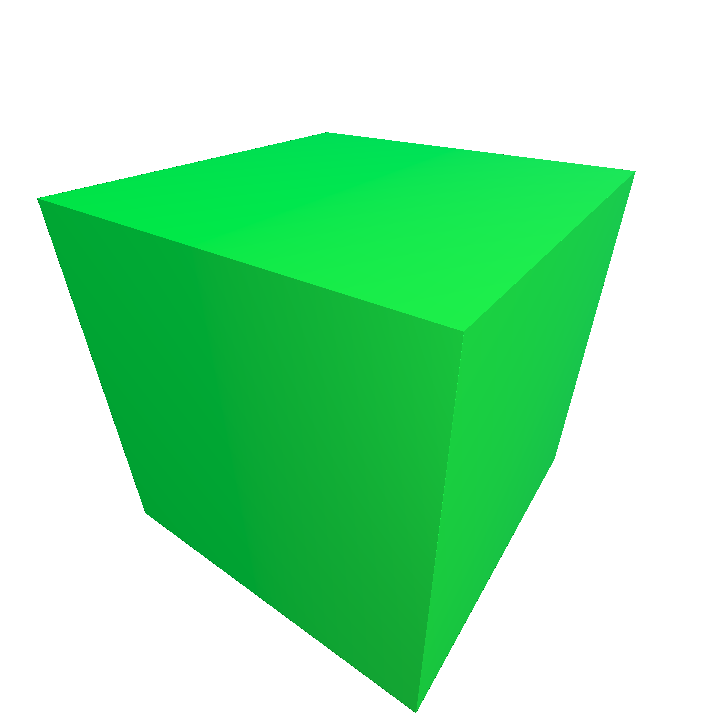
\includegraphics[width=\textwidth]{mengersponge0.png}
        \caption{}
        \label{fig:menger:sponge0}
    \end{subfigure}
    \hfill
    \begin{subfigure}[t]{0.11\textwidth}
        \centering
        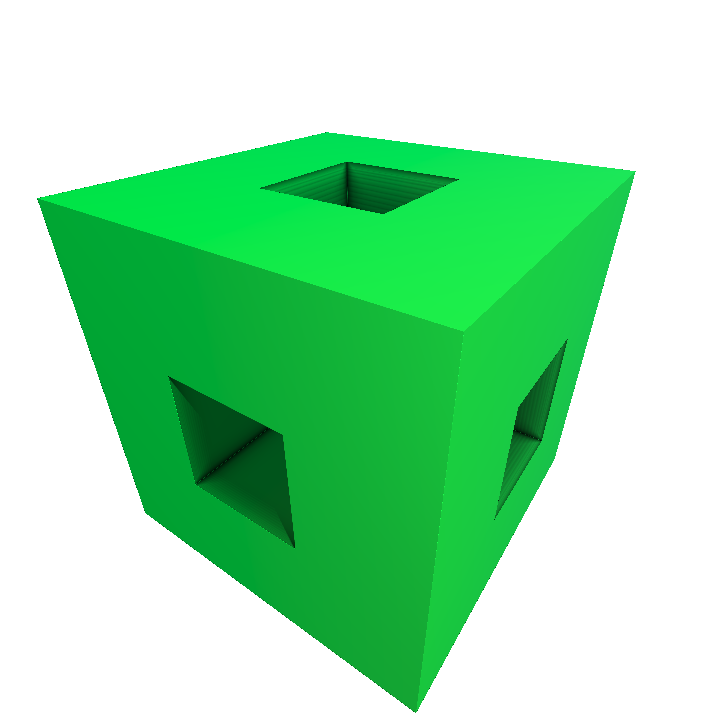
\includegraphics[width=\textwidth]{mengersponge1.png}
        \caption{}
        \label{fig:menger:sponge1}
    \end{subfigure}
    \hfill
    \begin{subfigure}[t]{0.11\textwidth}
        \centering
        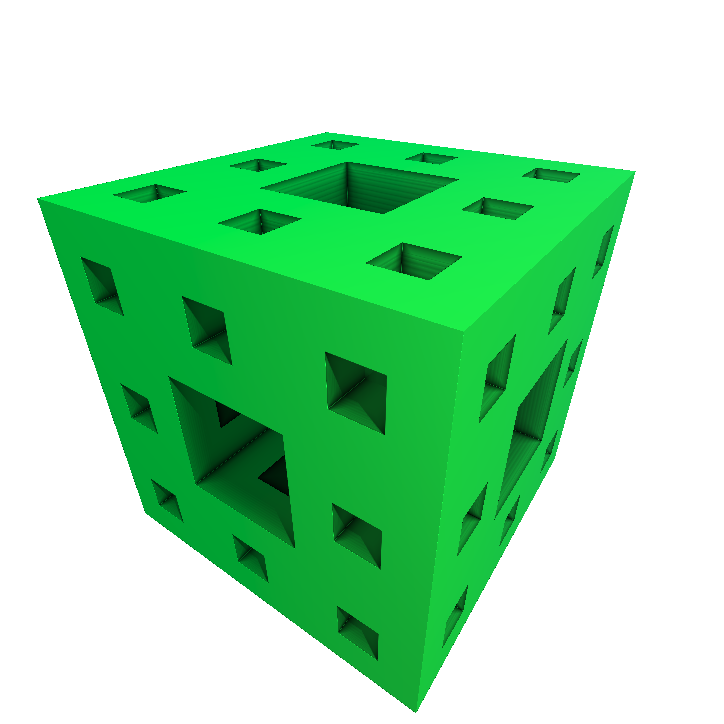
\includegraphics[width=\textwidth]{mengersponge2.png}
        \caption{}
        \label{fig:menger:sponge2}
    \end{subfigure}
    \hfill
    \begin{subfigure}[t]{0.11\textwidth}
        \centering
        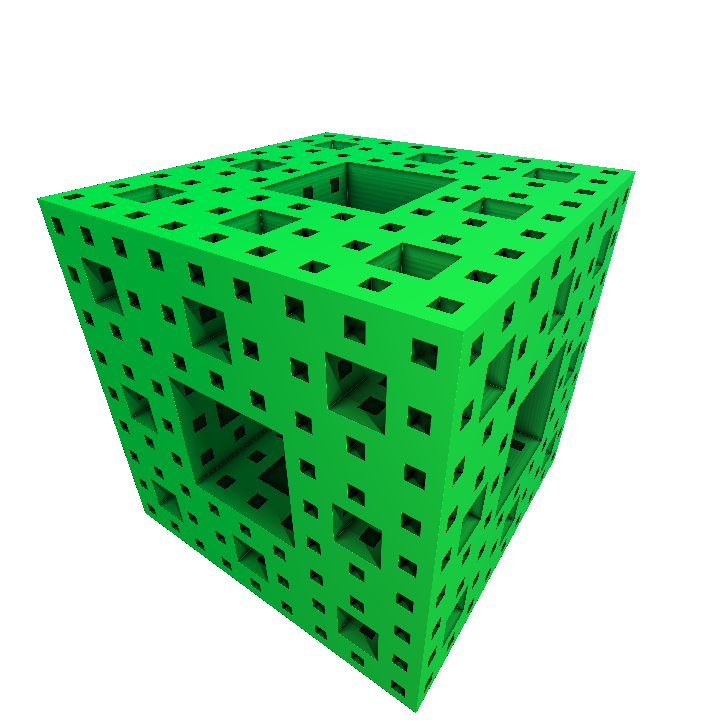
\includegraphics[width=\textwidth]{mengersponge3.png}
        \caption{}
        \label{fig:menger:sponge3}
    \end{subfigure}
    \begin{subfigure}[t]{0.11\textwidth}
        \centering
        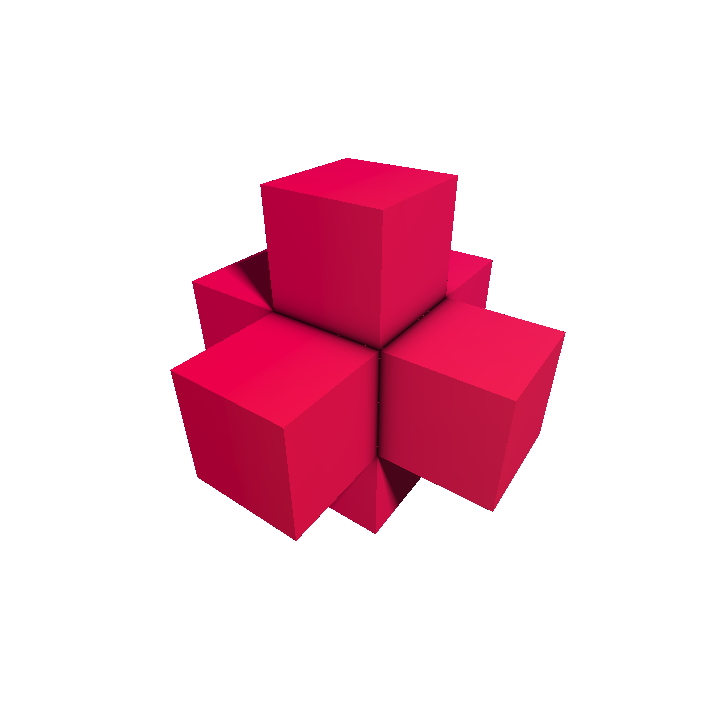
\includegraphics[width=\textwidth]{mengercross0.png}
        \caption{}
        \label{fig:menger:cross0}
    \end{subfigure}
    \hfill
    \begin{subfigure}[t]{0.11\textwidth}
        \centering
        
\includegraphics[width=\textwidth]{mengercross1.png}
        \caption{}
        \label{fig:menger:cross1}
    \end{subfigure}
    \hfill
    \begin{subfigure}[t]{0.11\textwidth}
        \centering
        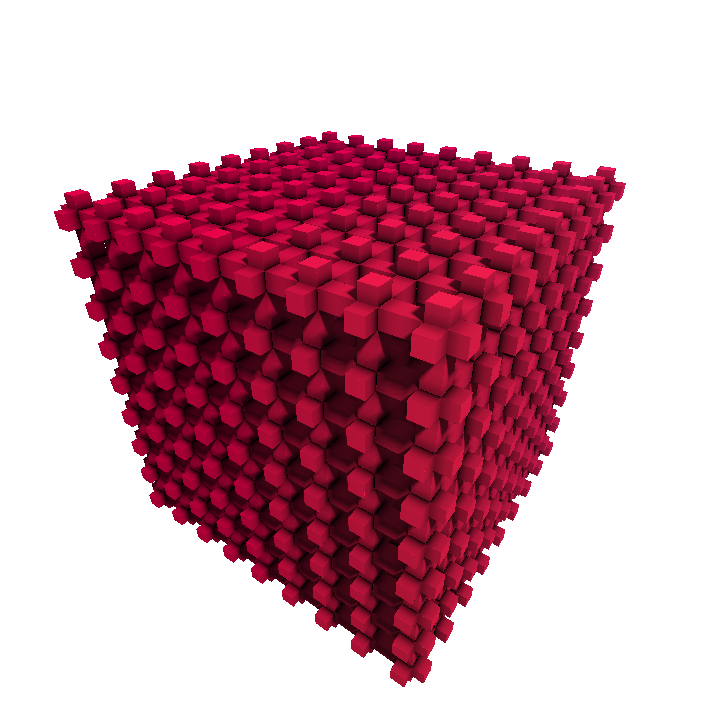
\includegraphics[width=\textwidth]{mengercross2.png}
        \caption{}
        \label{fig:menger:cross2}
    \end{subfigure}
    \begin{subfigure}[t]{0.11\textwidth}
        % subfigure used for alignment
        \centering
        
\includegraphics[width=\textwidth]{placeholder.png}
    \end{subfigure}
    \caption{Iterativ entstehender Menger-Sponge.}
    \label{fig:menger}
\end{figure}

\subsection{Interaktion mit dem Lenia-Mesh}
Der in Kapitel \ref{sec:lenia} besprochene Lenia-Algorithmus kann auf Mesh-Oberflächen angewendet werden.
Das in diesem Kapitel vorgestellte Ray-Marching-Verfahren stellt jedoch keine Mesh-Objekte dar.
Das in \autoref{fig:ray_and_mesh} gezeigte Ergebnis ergibt sich dadurch, dass es einen Shader für das Ray-Marching und einen für das Mesh-Objekt gibt.
Mit dem Ray-Marching-Shader kann eine Environment-Map erzeugt werden, die im Mesh-Shader für die Reflexionen verwendet wird.
Wenn der Depth-Buffer beider Fragment-Shader entsprechend angepasst wird, ist es auch möglich, dass ein Objekt aus dem einen Shader das Objekt aus dem anderen Shader verdeckt.
Auf die bei der Implementierung zu beachtenden Details wird in diesem Bericht nicht weiter eingegangen.

\begin{figure}[!htbp]\centering
    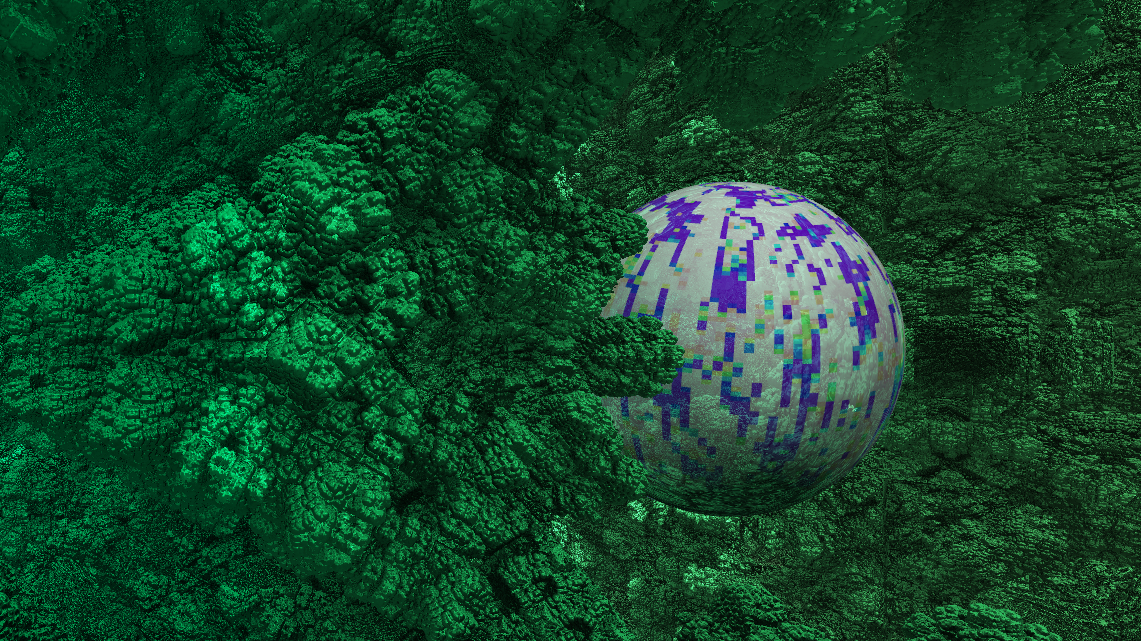
\includegraphics[width=0.5\textwidth - 7.82454pt]{overlap_cropped_bright.png}
    \caption{Überschneidung von Mesh-Objekt mit Ray-Marching Objekt und Reflexion.}
    \label{fig:ray_and_mesh}
\end{figure}

